\section{Cylinder Hitting a Wall} \label{sec:cylHittingWall}

In this example a cylinder of mass $M=100$, radius $R=.5$, initial centre of mass at $\xv=0$,
is impulsively started with a velocity $\uv=(1,0)$. The cylinder is directed towards a
a no-slip wall located at $x=2.$. 

{
\newcommand{\figWidth}{.75\linewidth}
\begin{figure}
\begin{center}
%
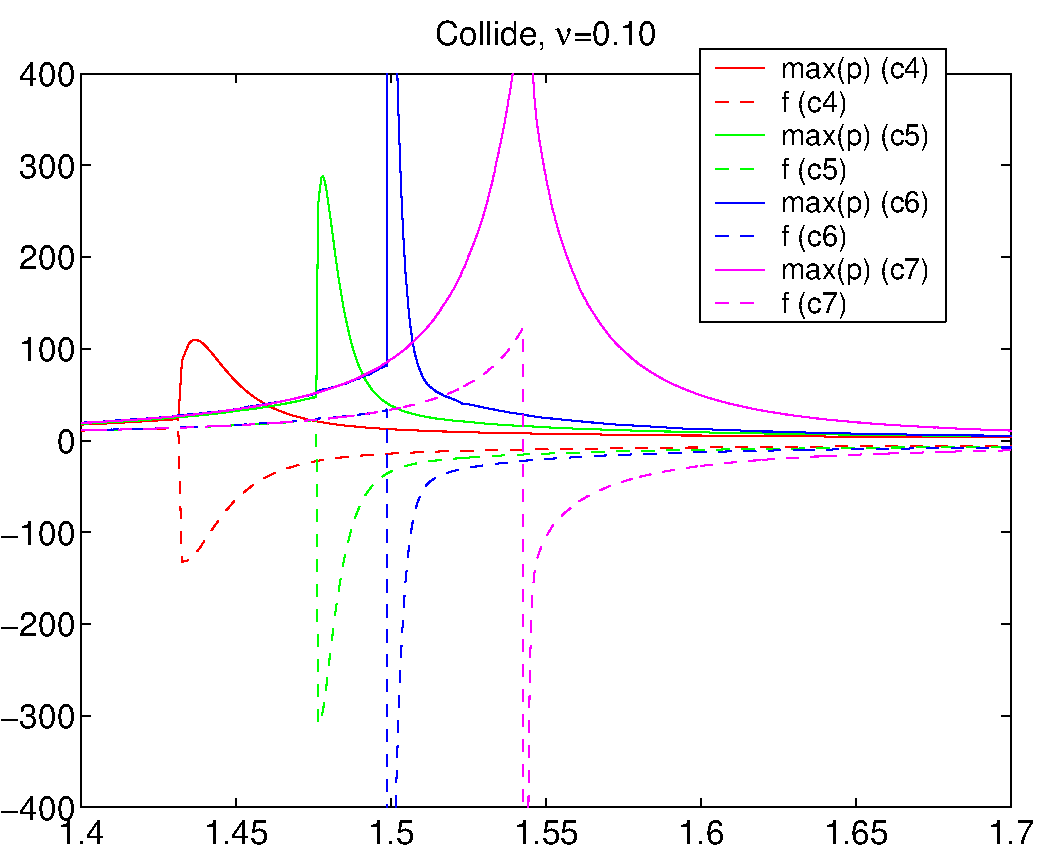
\includegraphics[width=\figWidth]{figures/collide-nu0p1}  
%
\end{center}
\caption{Cylinder hitting a wall, $\nu=.1$} 
\end{figure}
}

{
\newcommand{\figWidth}{.32\linewidth}
\begin{figure}
\begin{center}
%
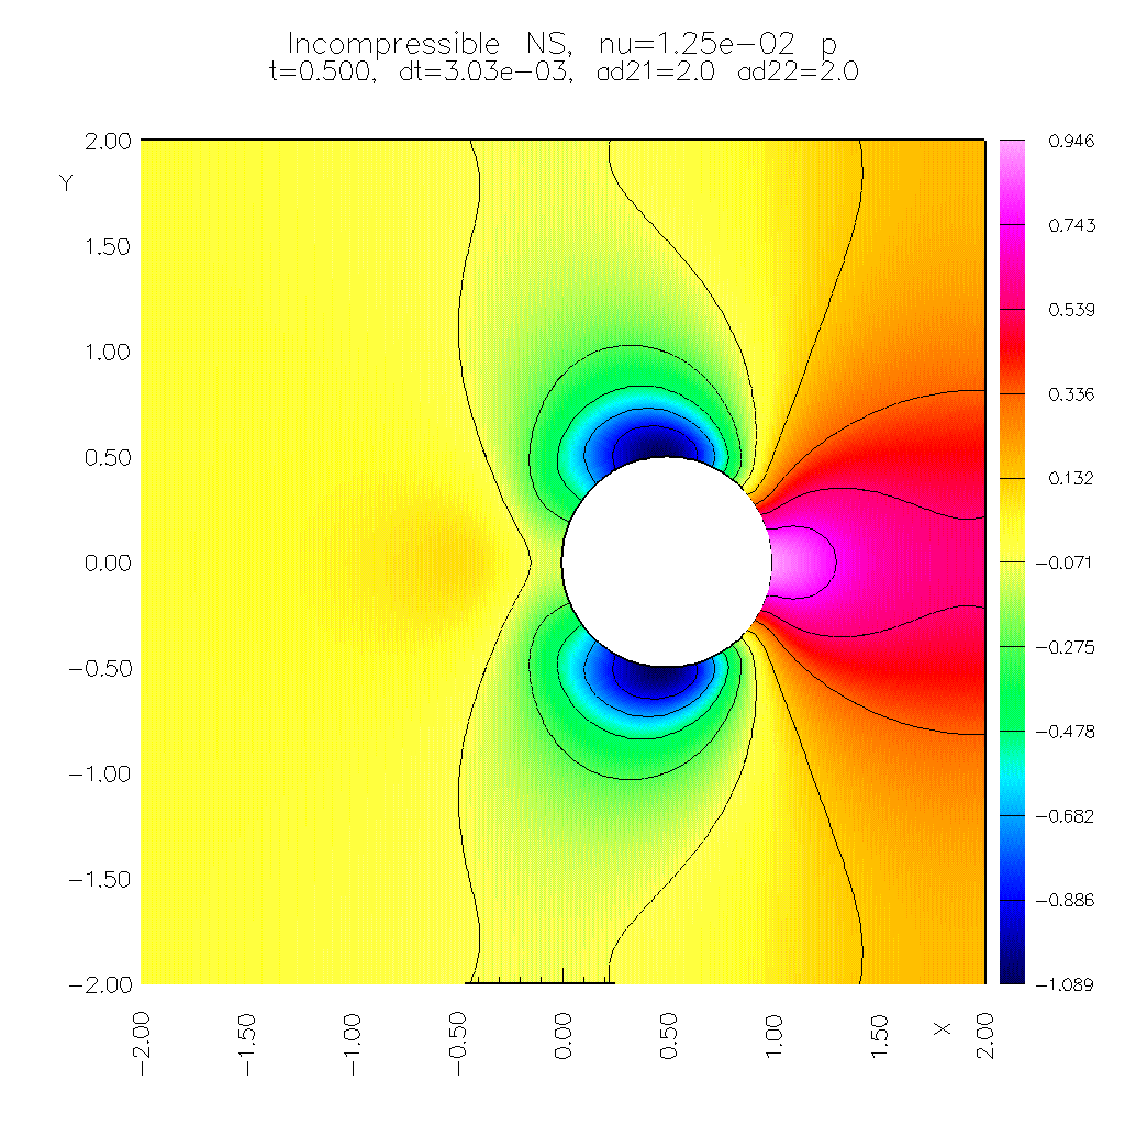
\includegraphics[width=\figWidth]{figures/collide5-p-0p5}  
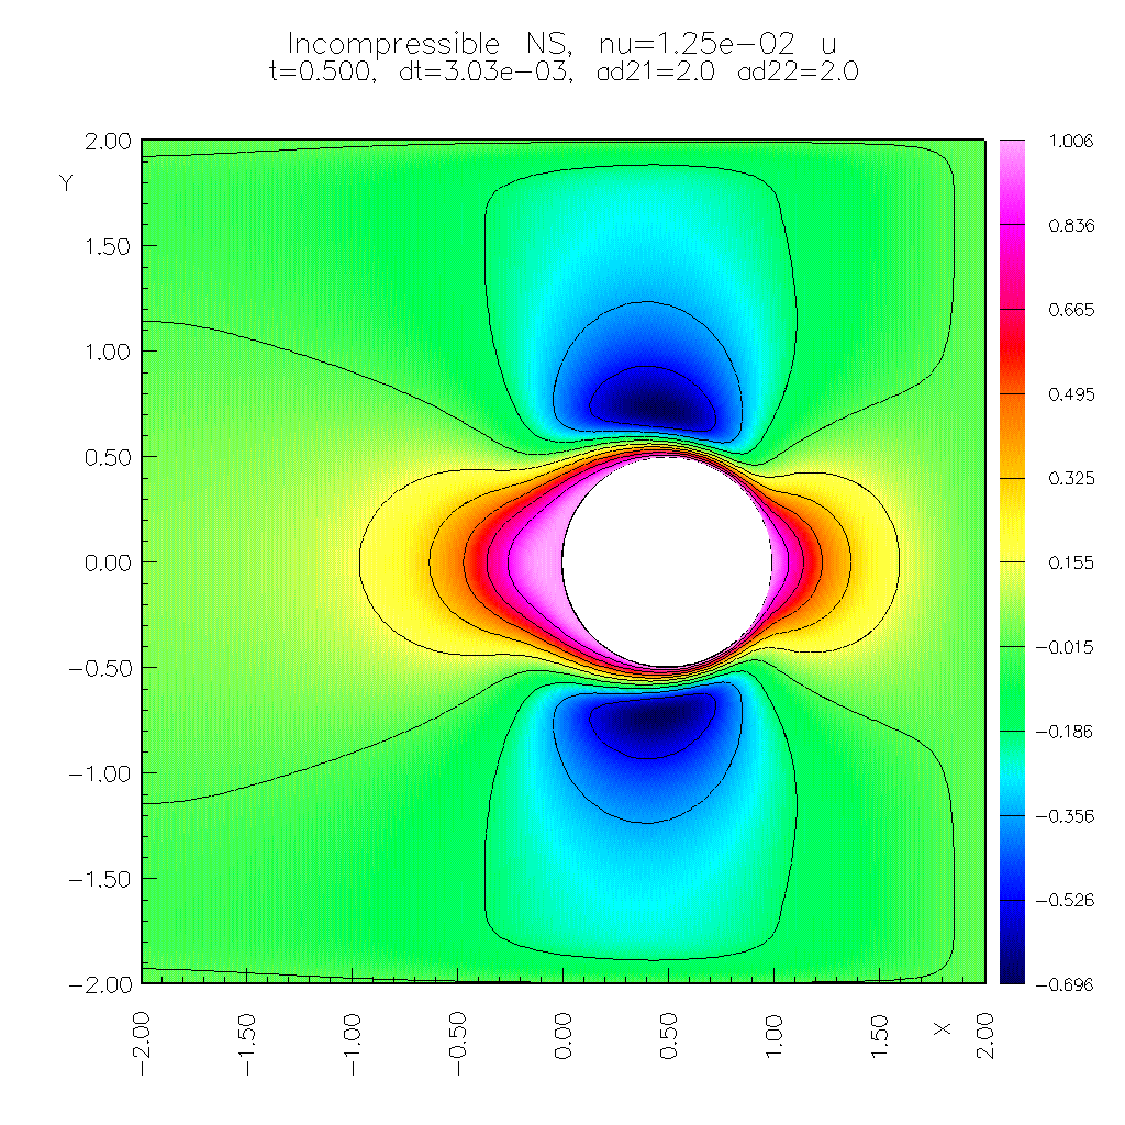
\includegraphics[width=\figWidth]{figures/collide5-u-0p5}  
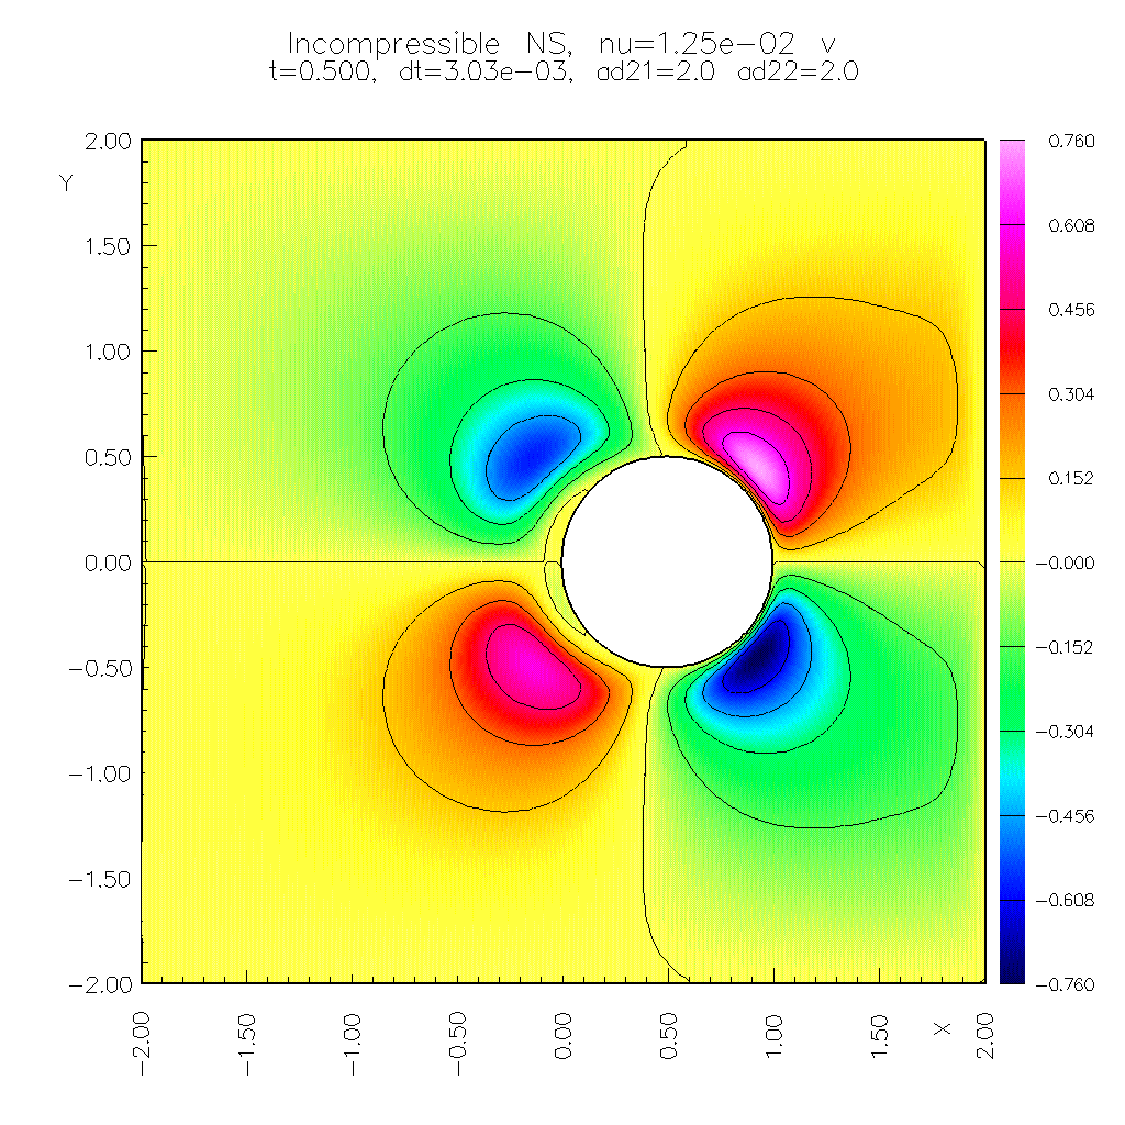
\includegraphics[width=\figWidth]{figures/collide5-v-0p5}  
%
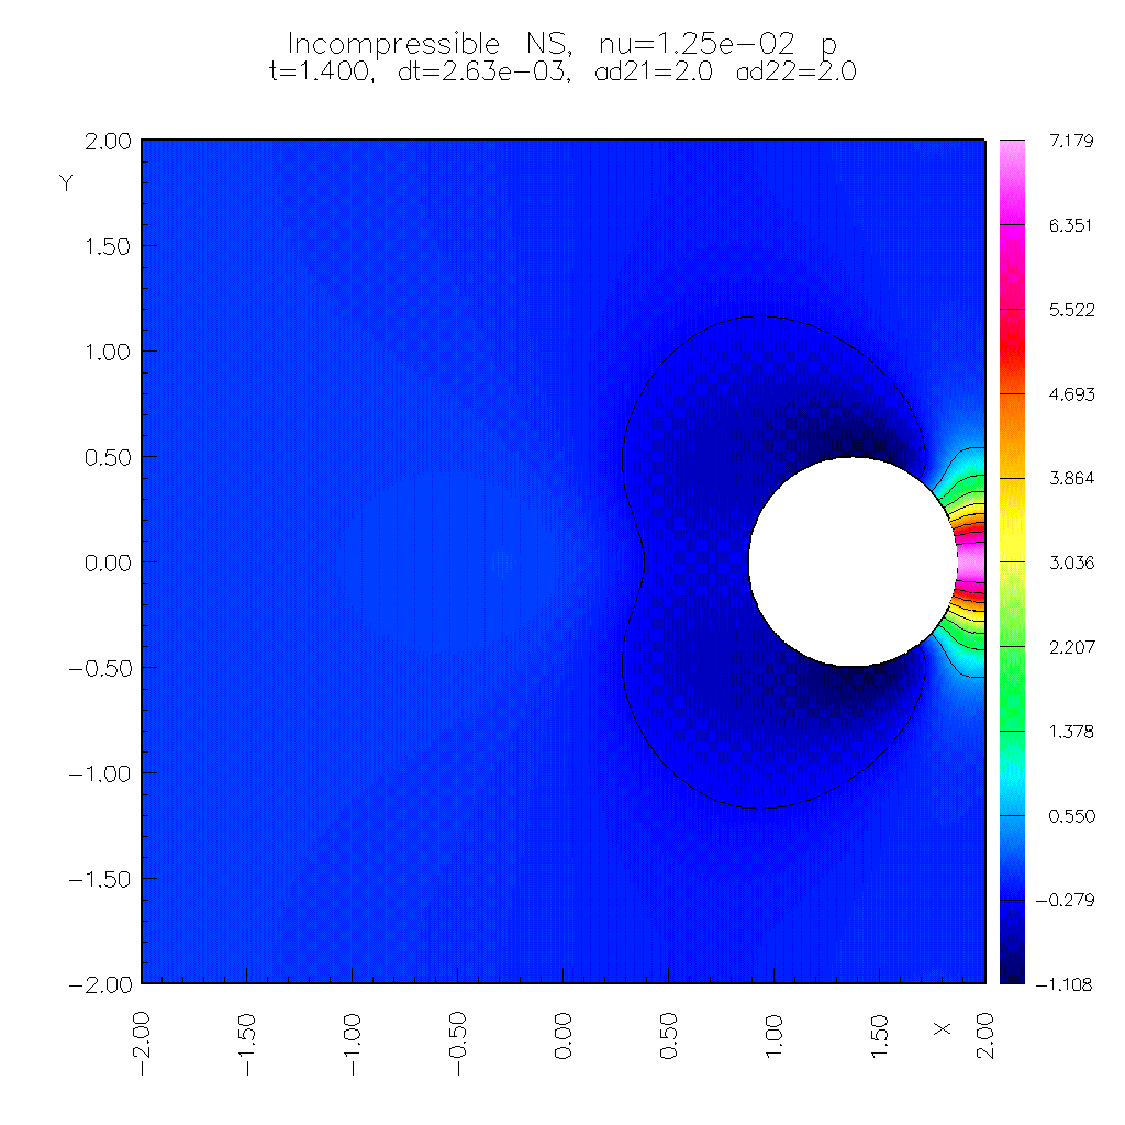
\includegraphics[width=\figWidth]{figures/collide5-p-1p4}  
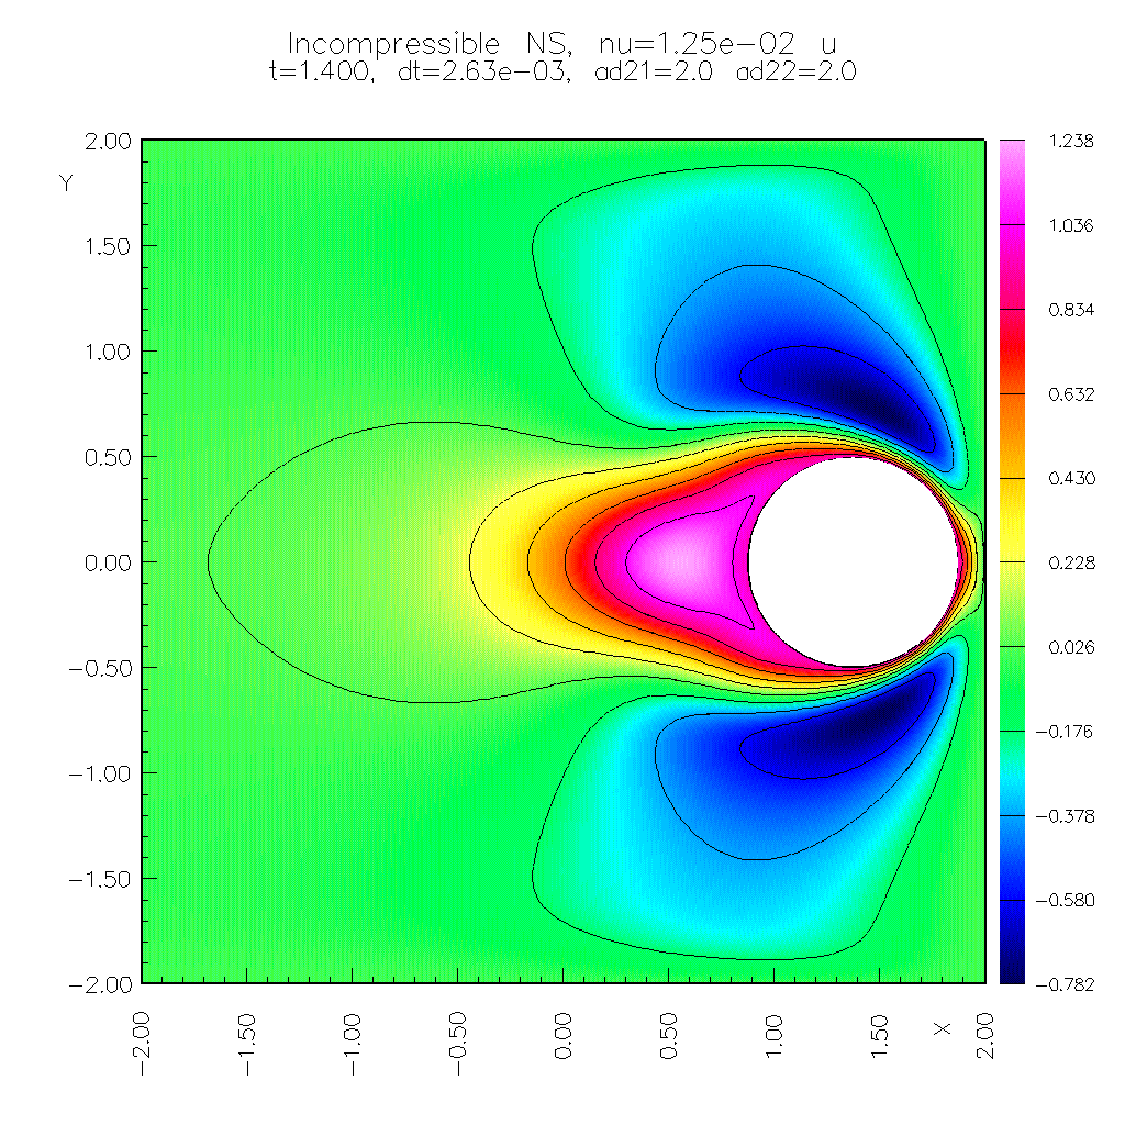
\includegraphics[width=\figWidth]{figures/collide5-u-1p4}  
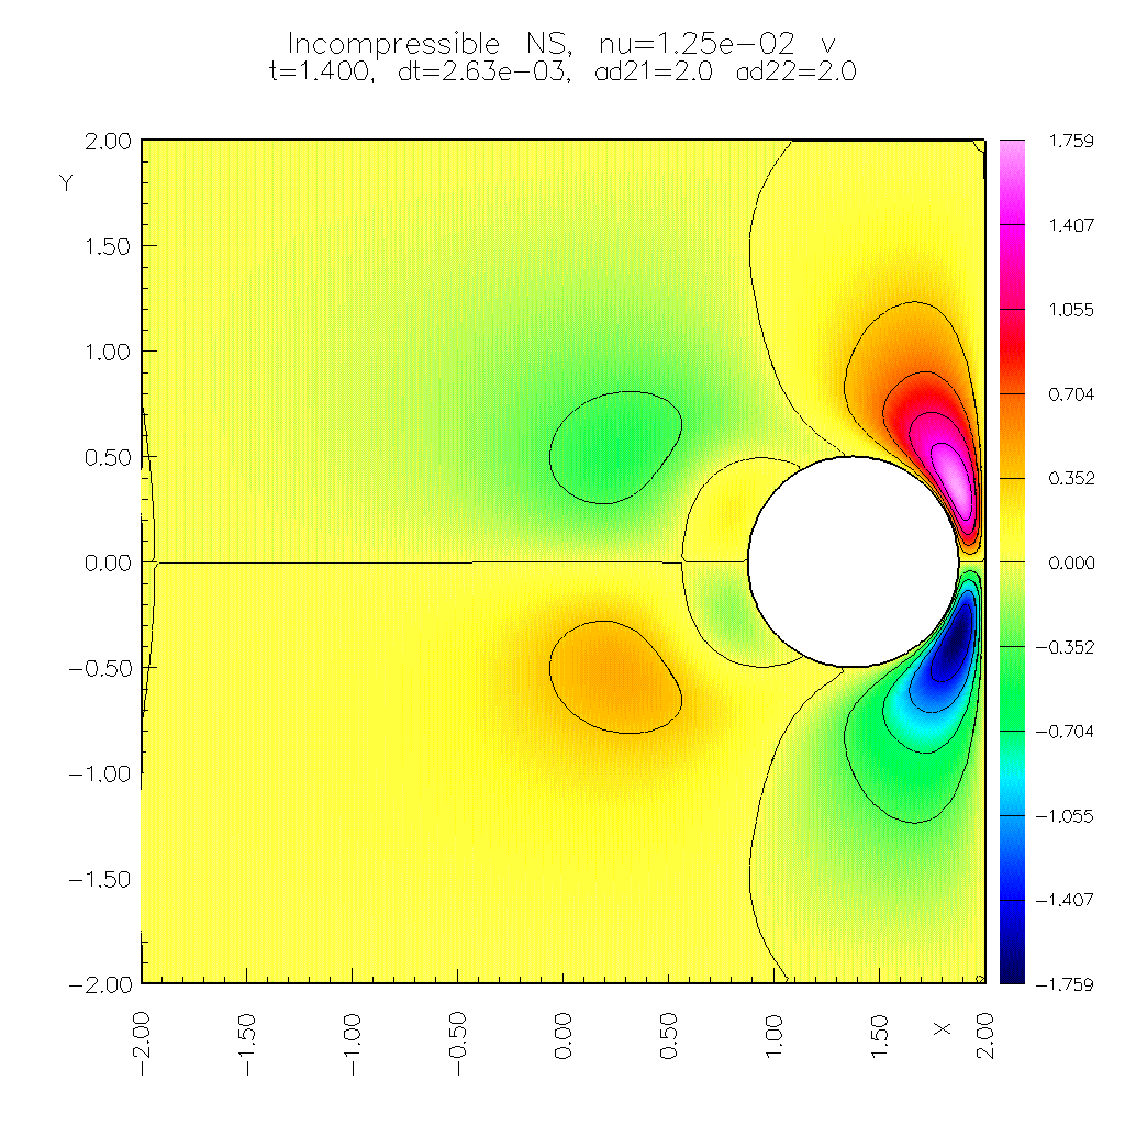
\includegraphics[width=\figWidth]{figures/collide5-v-1p4}  
%
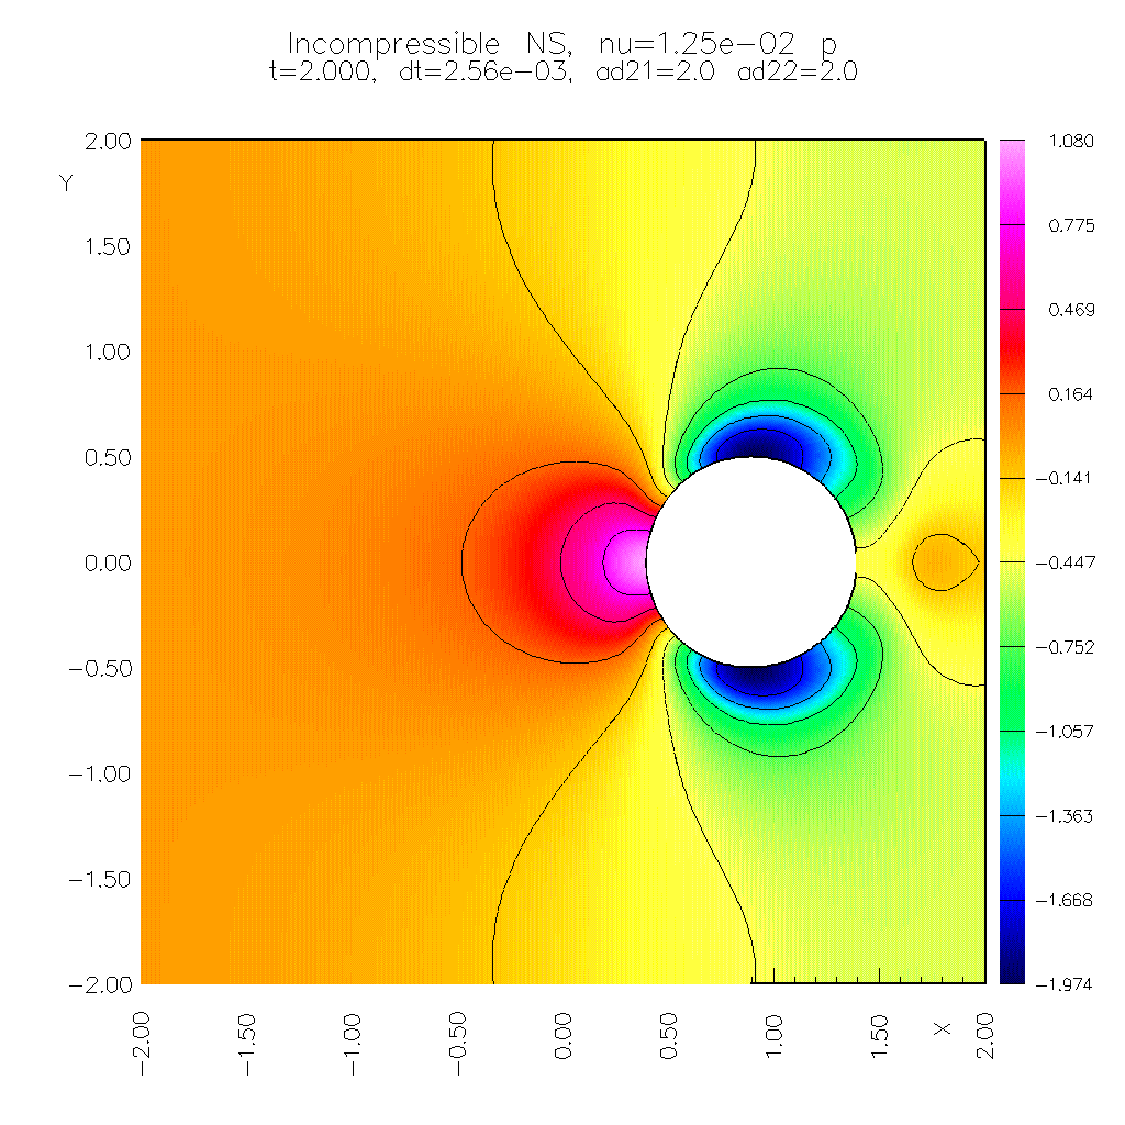
\includegraphics[width=\figWidth]{figures/collide5-p-2p0}  
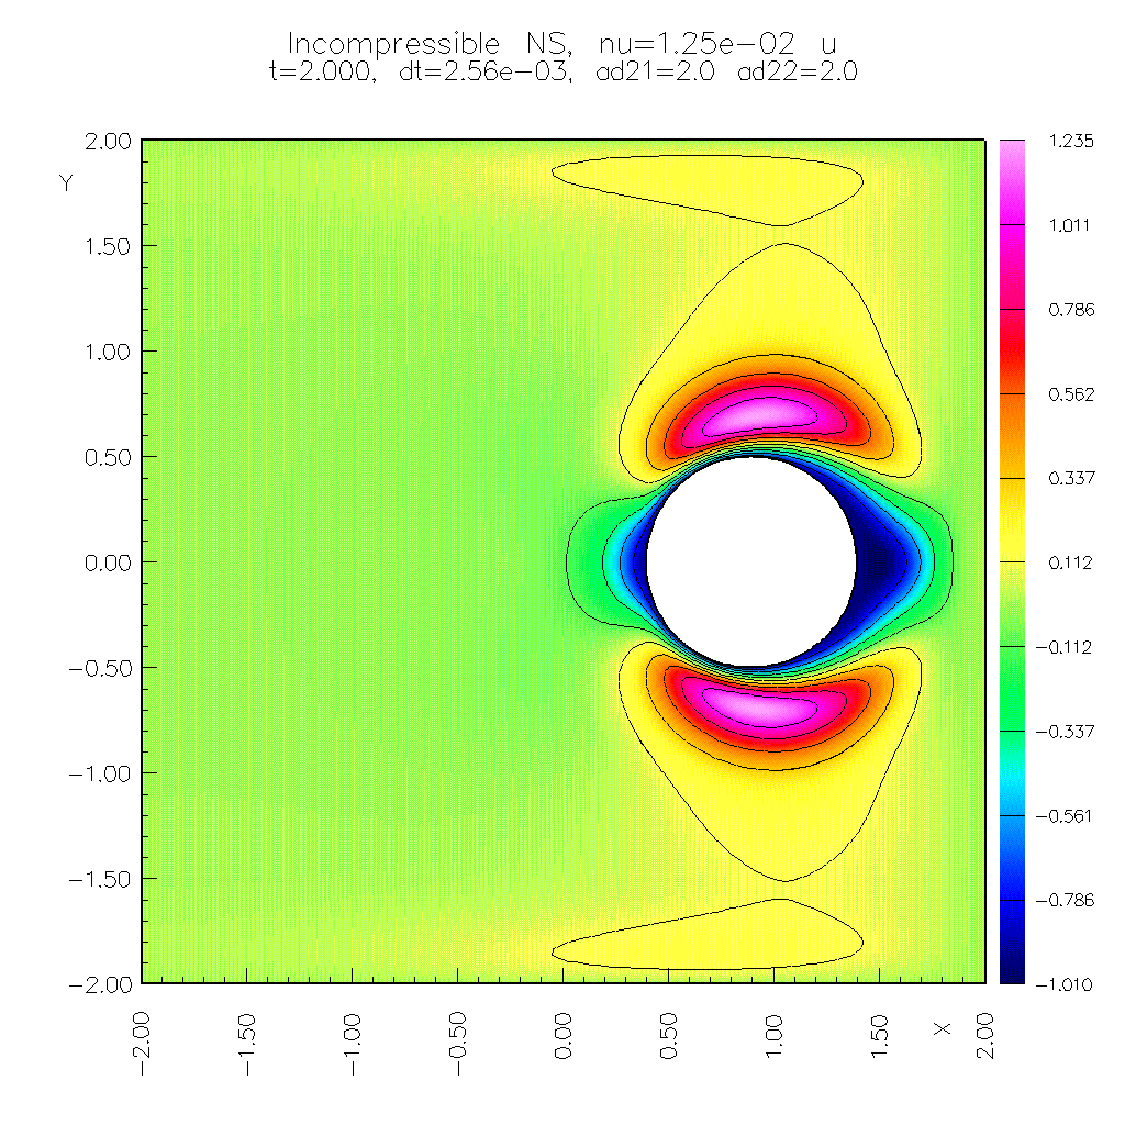
\includegraphics[width=\figWidth]{figures/collide5-u-2p0}  
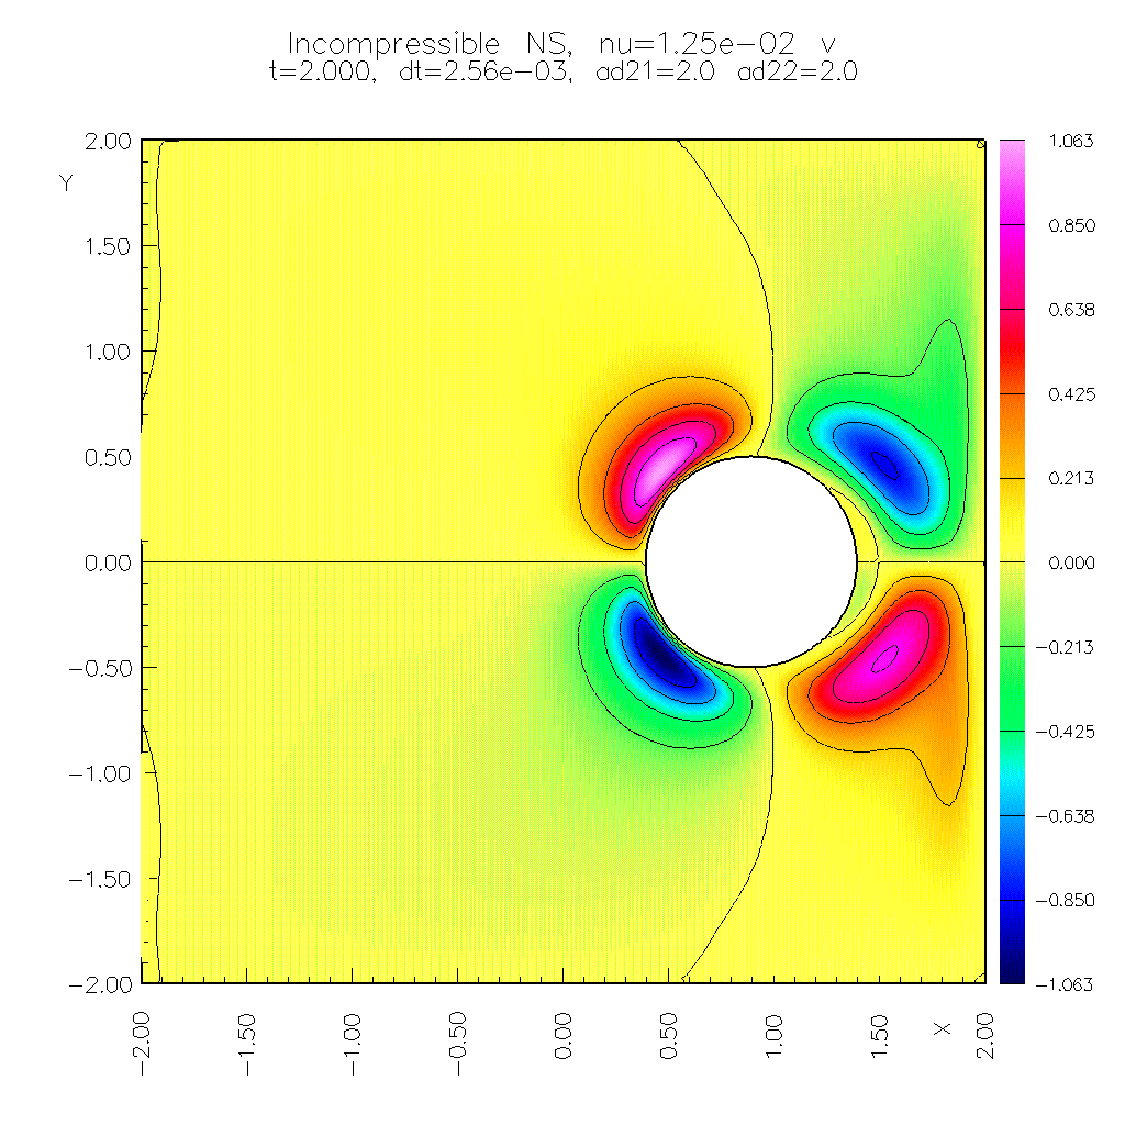
\includegraphics[width=\figWidth]{figures/collide5-v-2p0}  
\end{center}
\caption{Cylinder hitting a wall, $\nu=.0125$, solution at times $.5$, $1.4$ and $2.0$} 
\end{figure}
}

{
\newcommand{\figWidth}{.45\linewidth}
\begin{figure}
\begin{center}
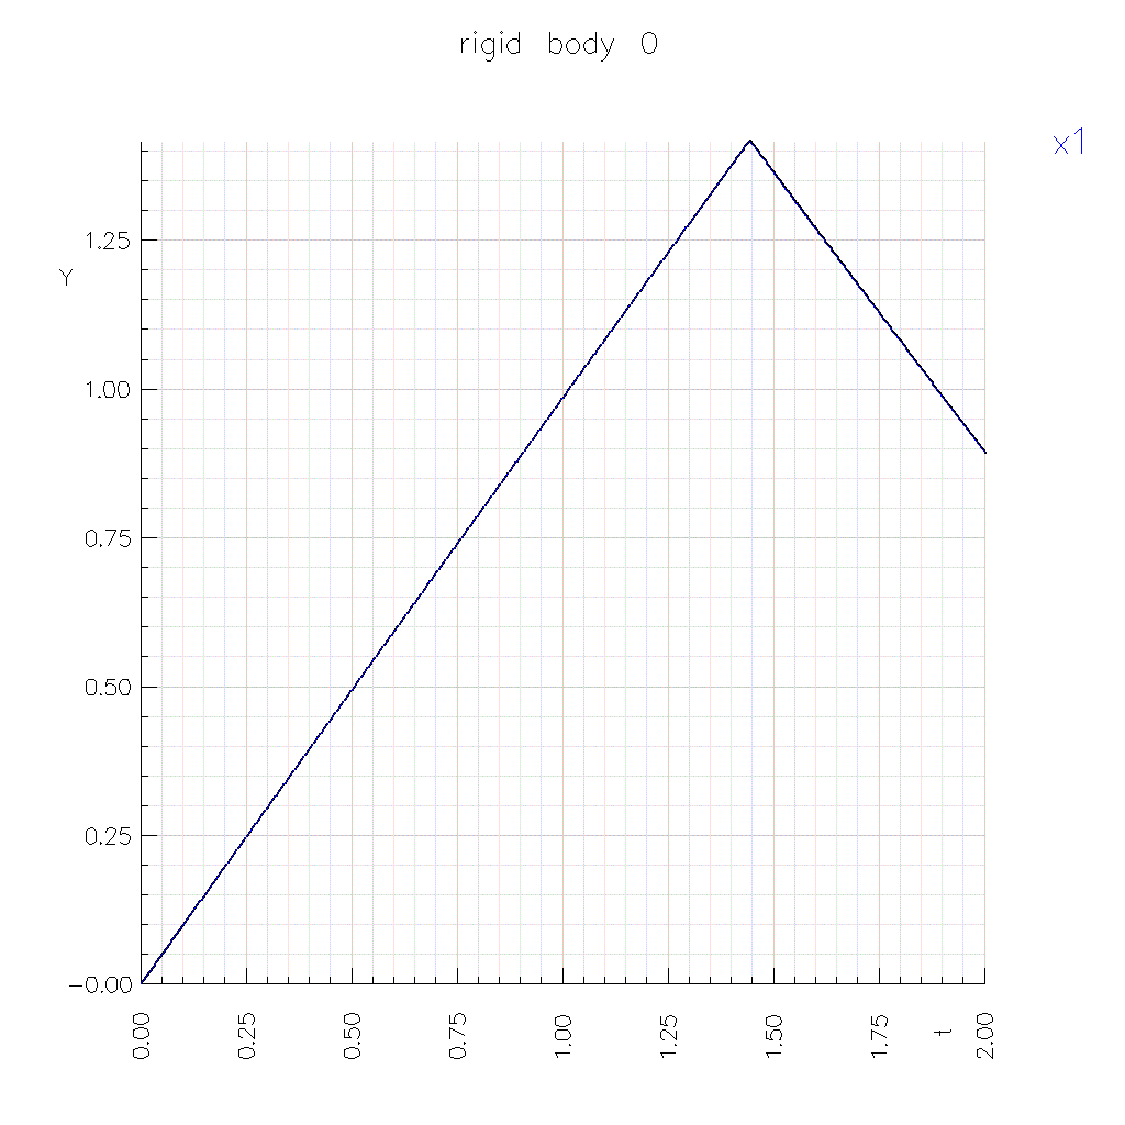
\includegraphics[width=\figWidth]{figures/collide5-rb-x1}  
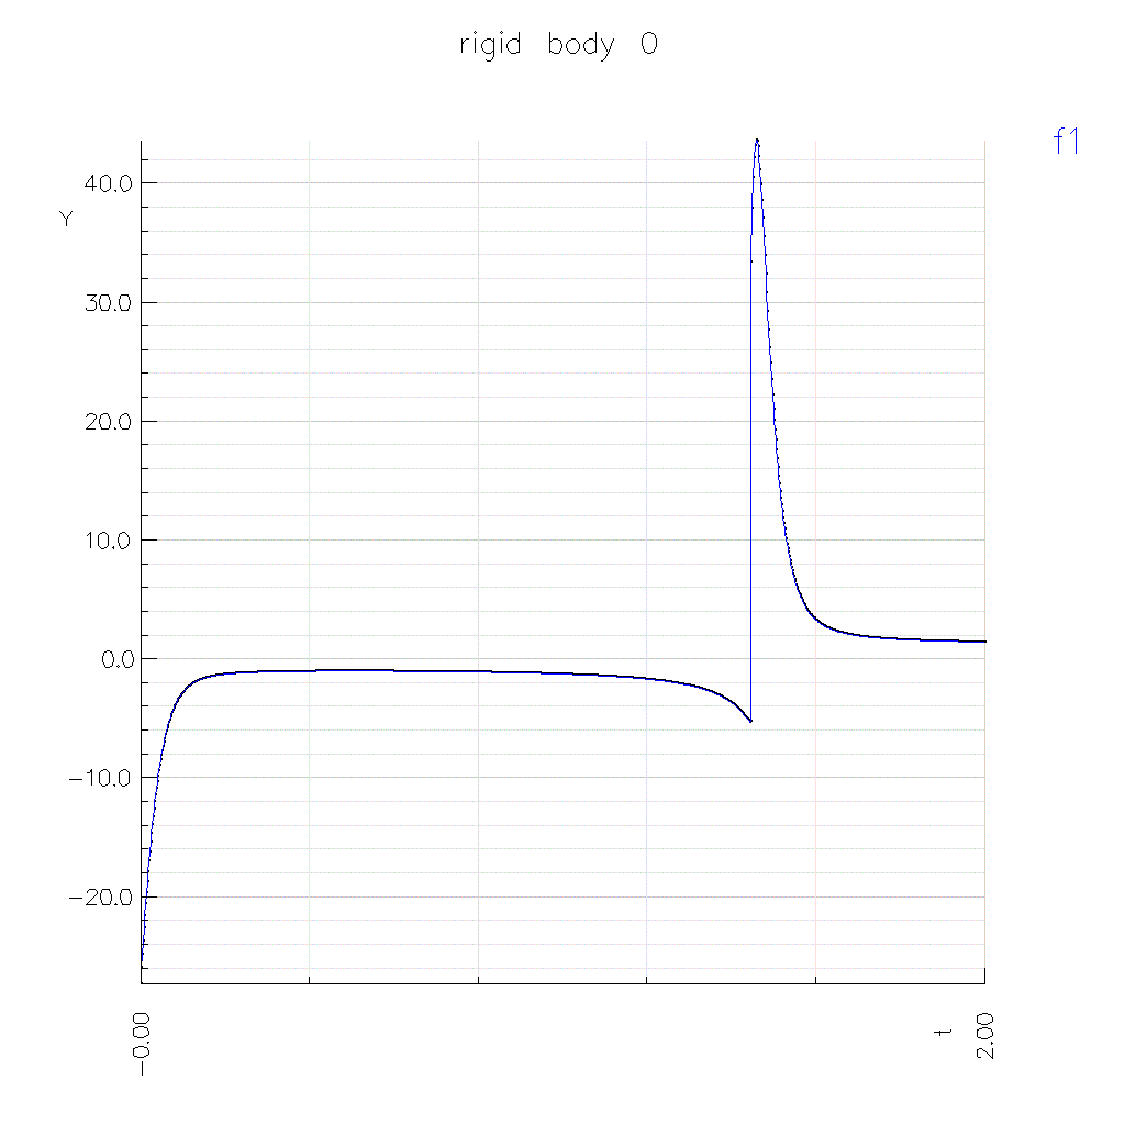
\includegraphics[width=\figWidth]{figures/collide5-rb-f1}  
% 
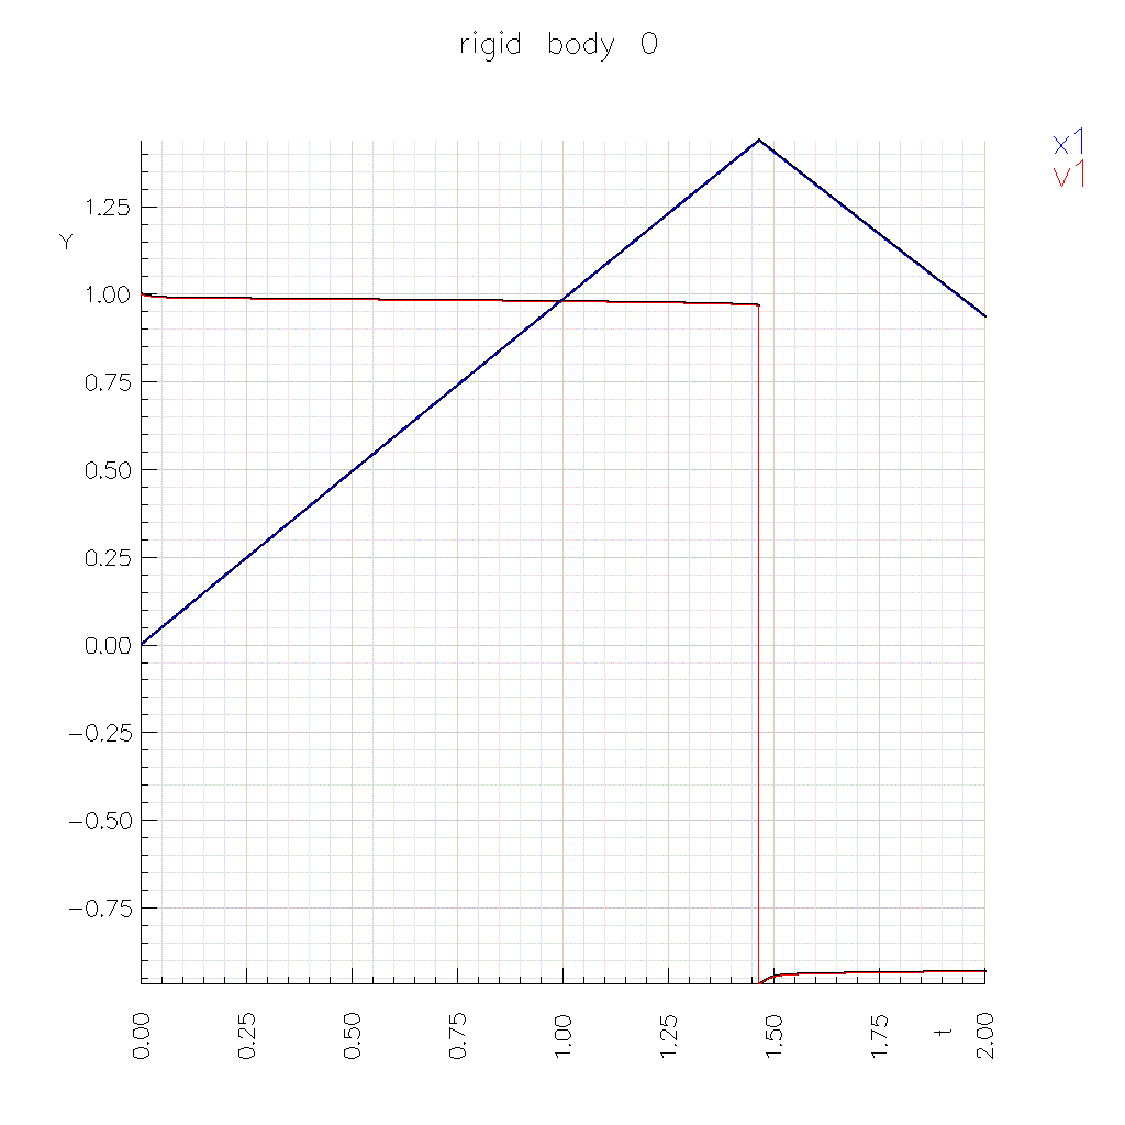
\includegraphics[width=\figWidth]{figures/collide6-nu0125-rb-x1}  
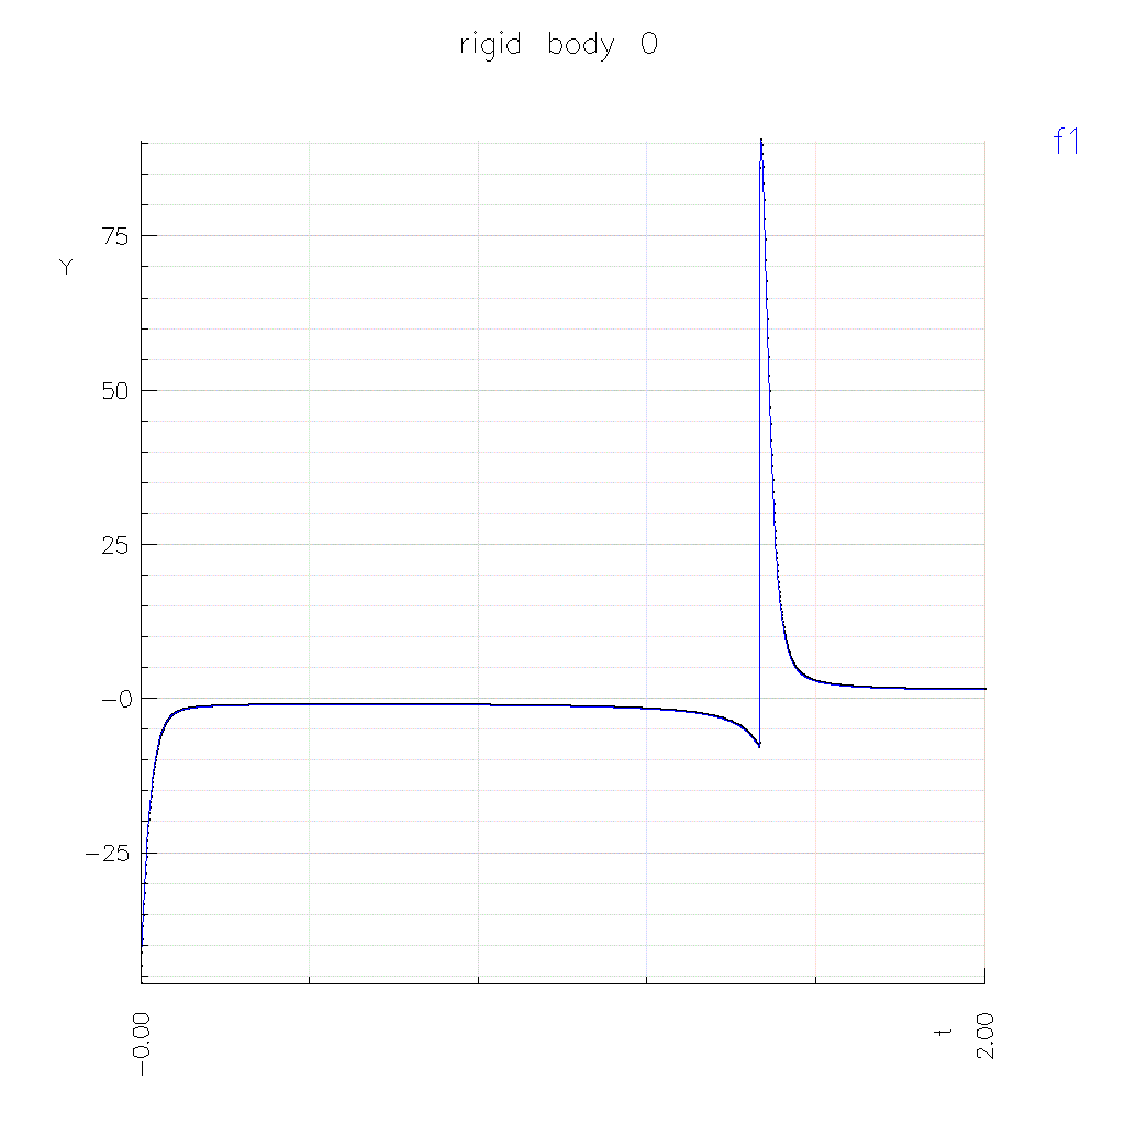
\includegraphics[width=\figWidth]{figures/collide6-nu0125-rb-f1}  
\end{center}
\caption{Cylinder hitting a wall, $\nu=.005$, position of the centre of mass and the force on the cylinder.
    Top: grid cic5, bottom grid cic6.}
\end{figure}
}

% ---------------------------------------------------------------------------

{
\newcommand{\figWidth}{.32\linewidth}
\begin{figure}
\begin{center}
%
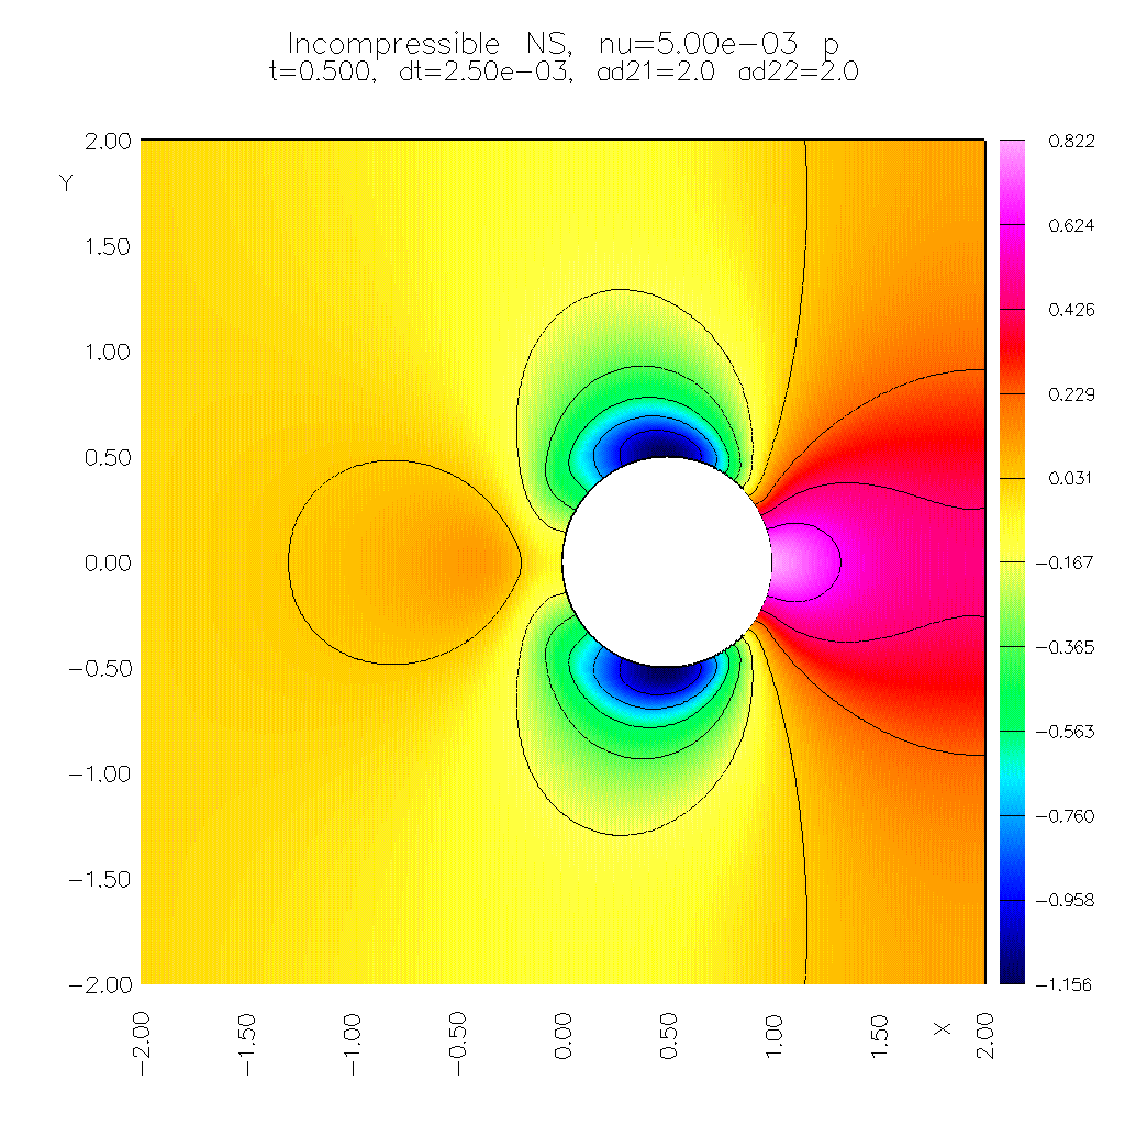
\includegraphics[width=\figWidth]{figures/collide6-p-0p5}  
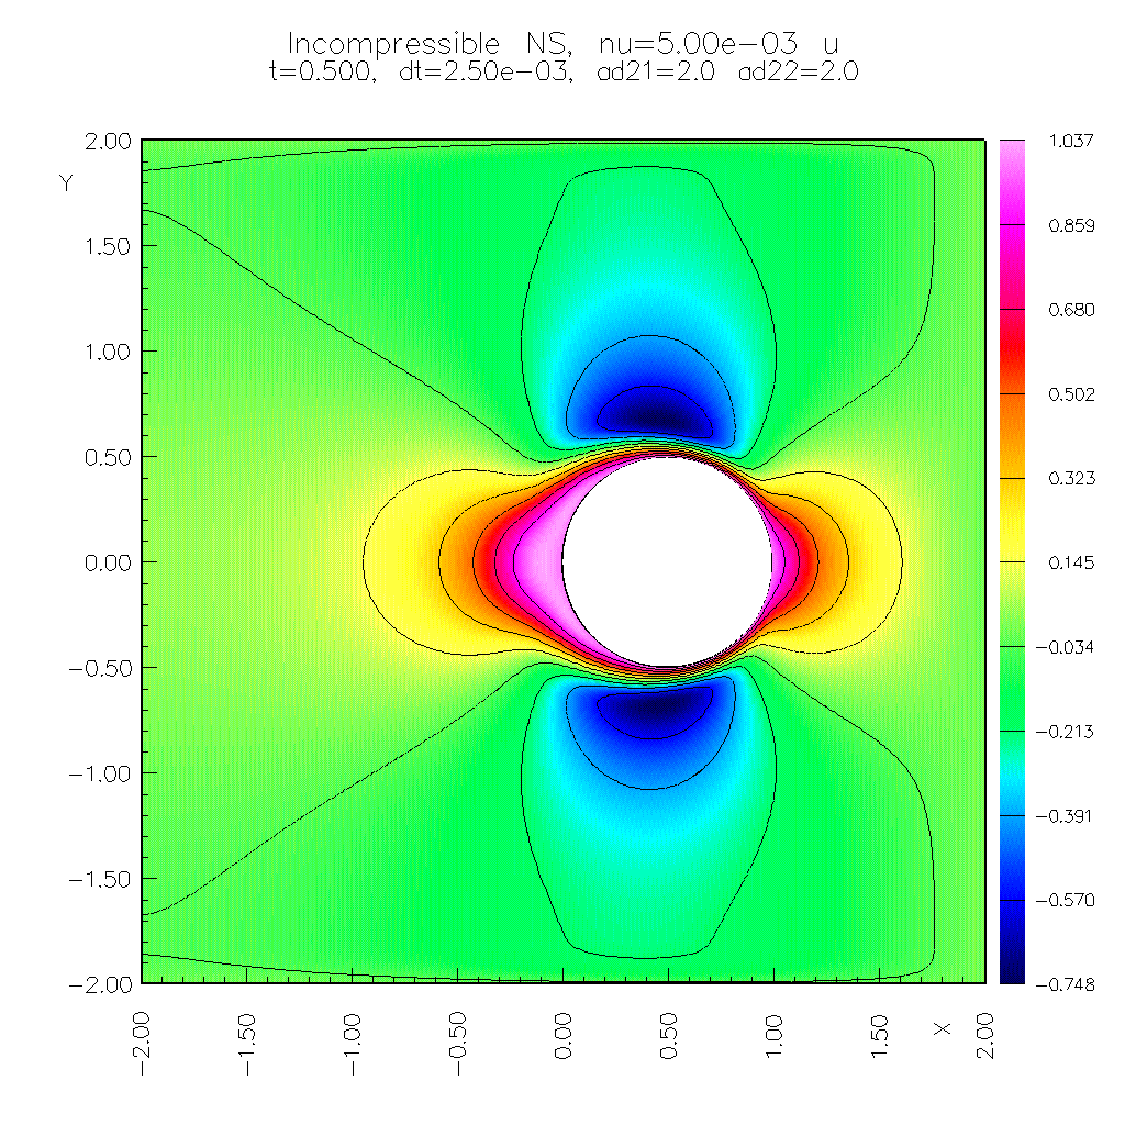
\includegraphics[width=\figWidth]{figures/collide6-u-0p5}  
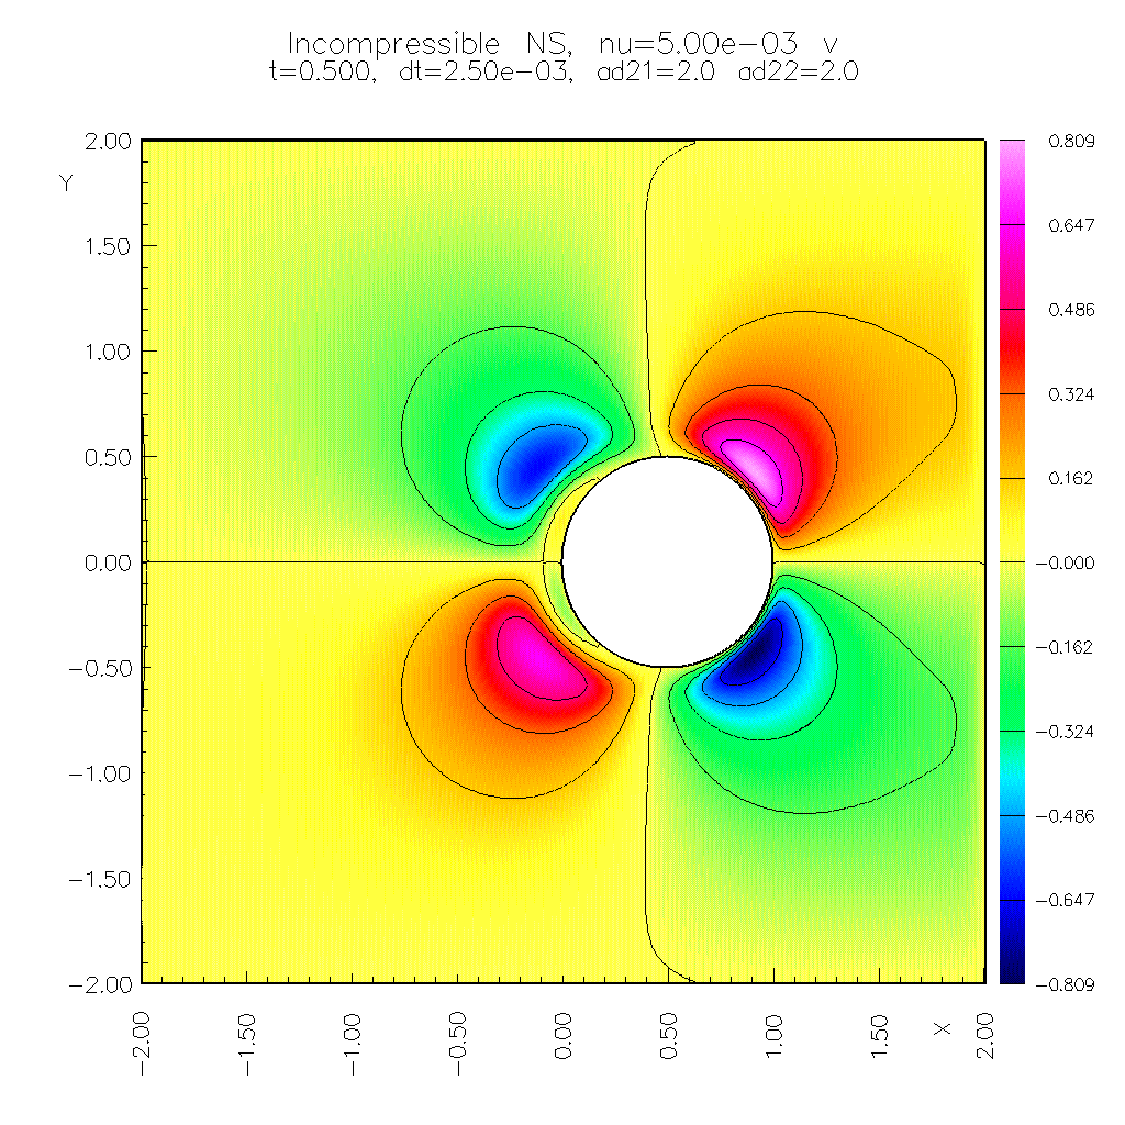
\includegraphics[width=\figWidth]{figures/collide6-v-0p5}  
%
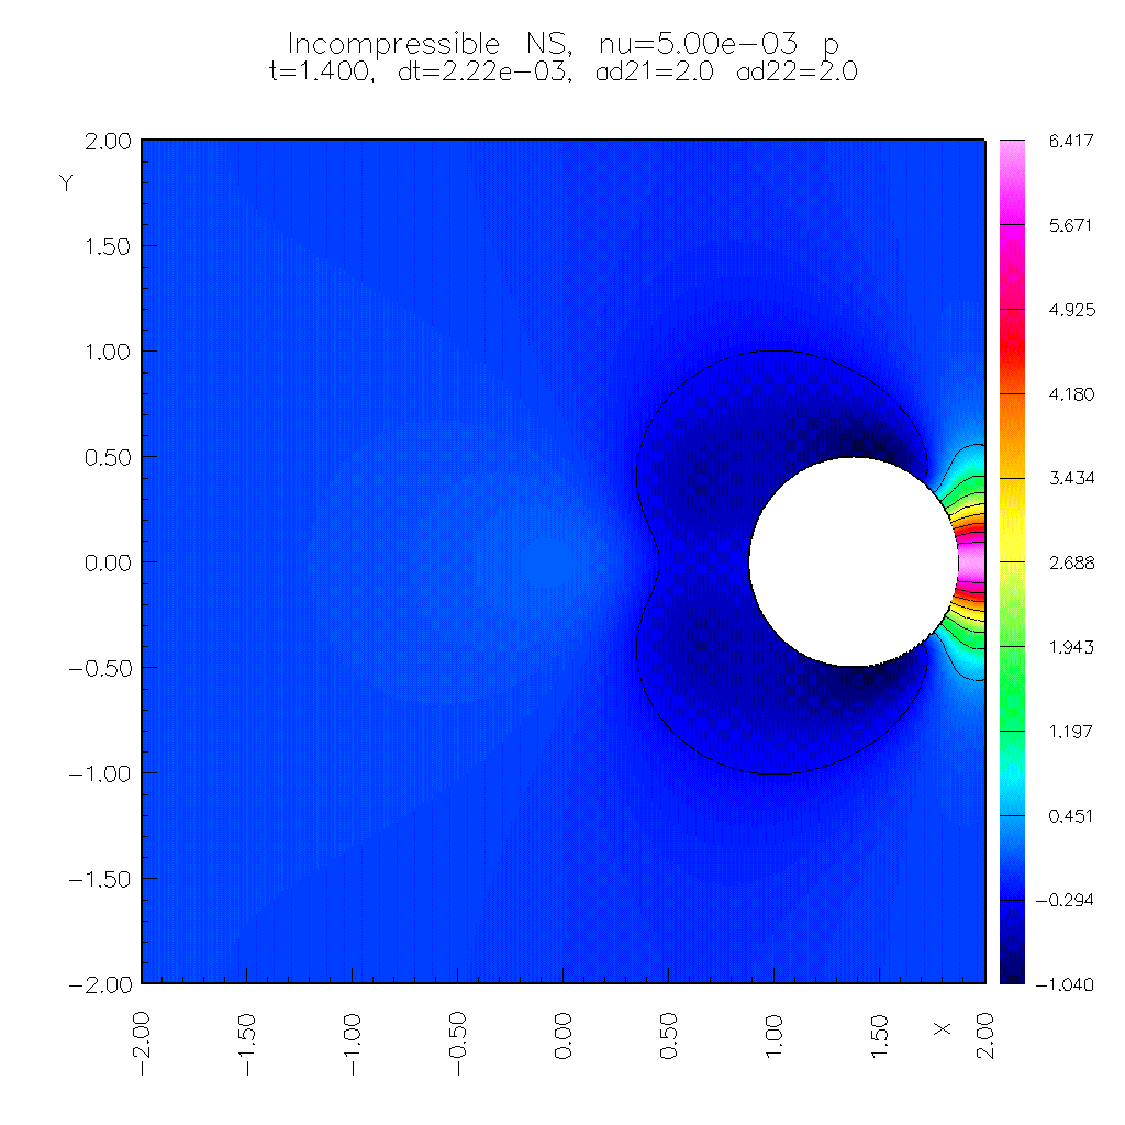
\includegraphics[width=\figWidth]{figures/collide6-p-1p4}  
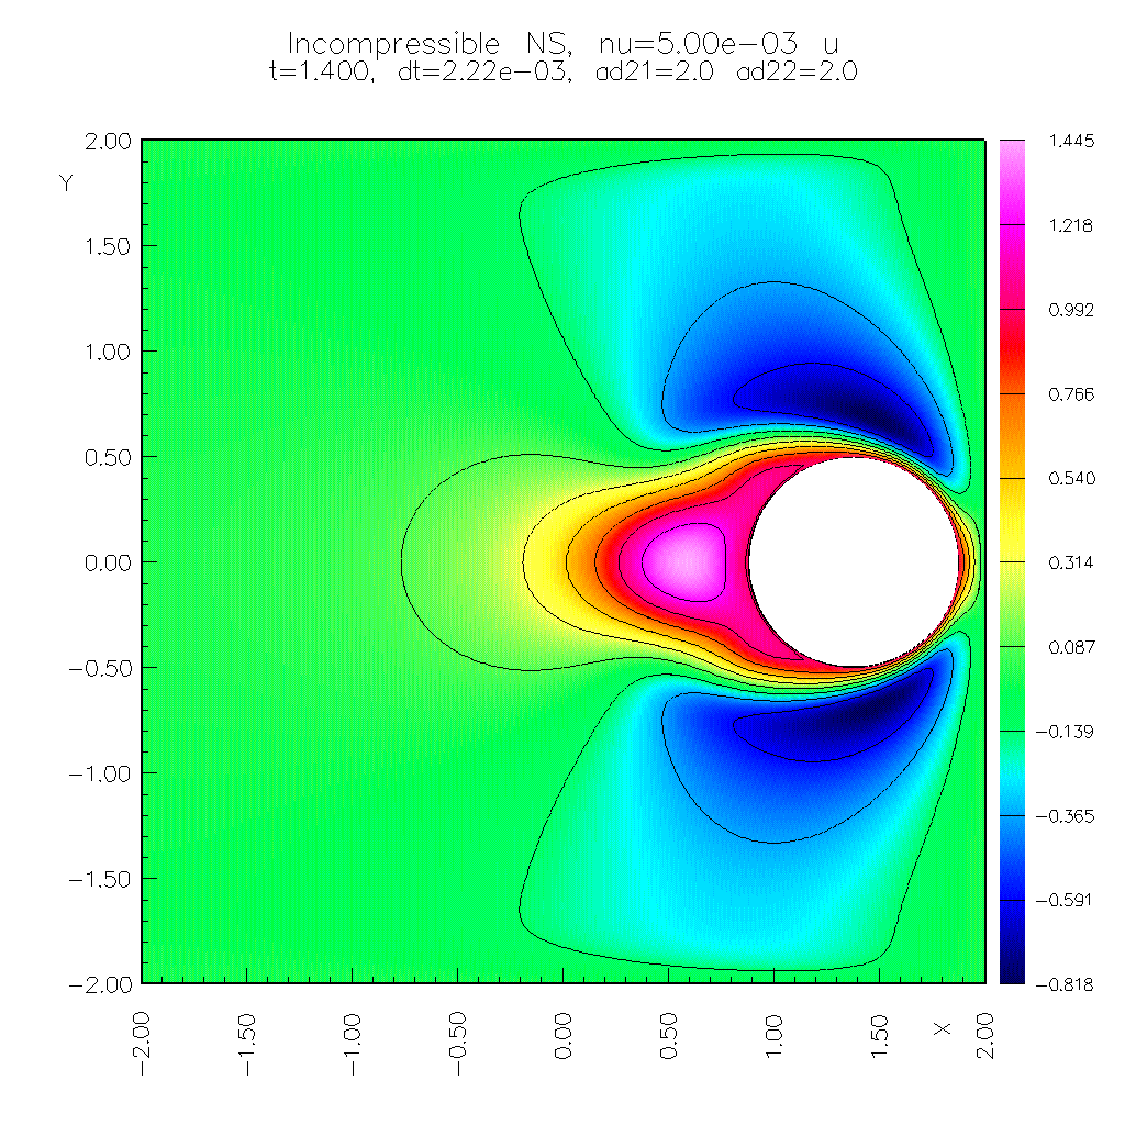
\includegraphics[width=\figWidth]{figures/collide6-u-1p4}  
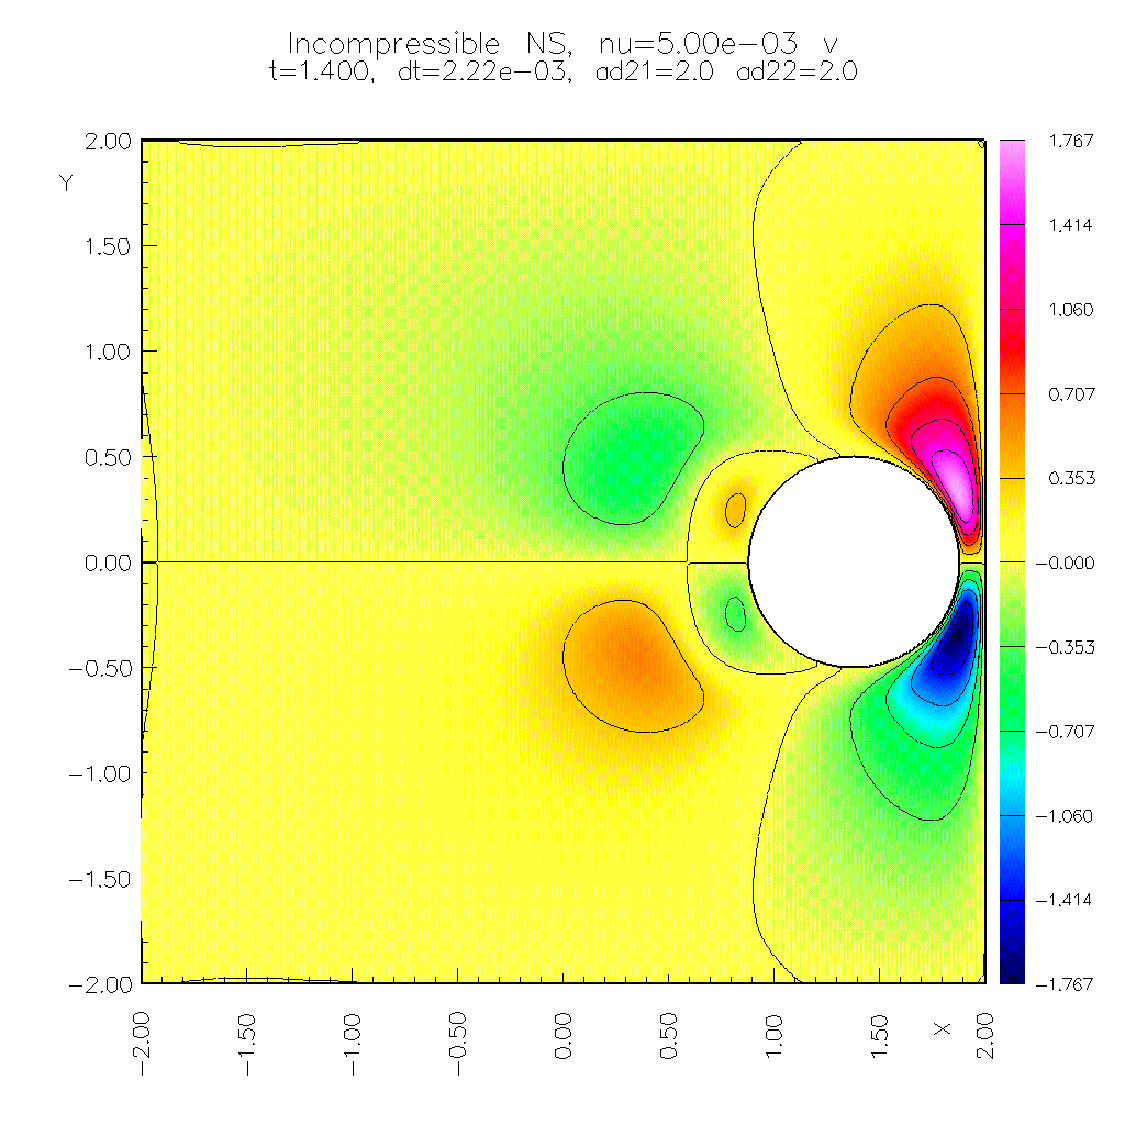
\includegraphics[width=\figWidth]{figures/collide6-v-1p4}  
%
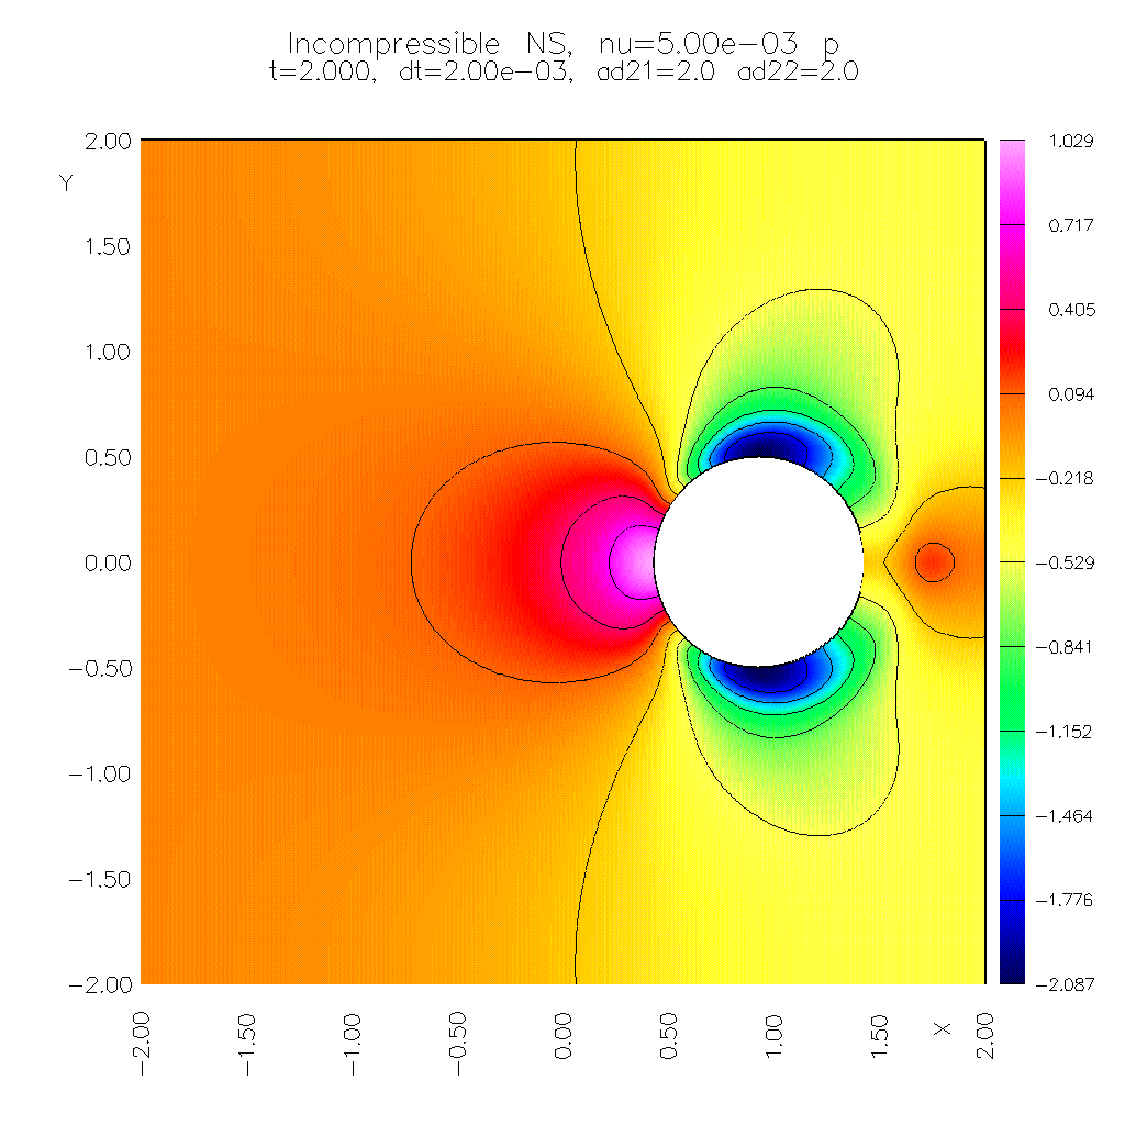
\includegraphics[width=\figWidth]{figures/collide6-p-2p0}  
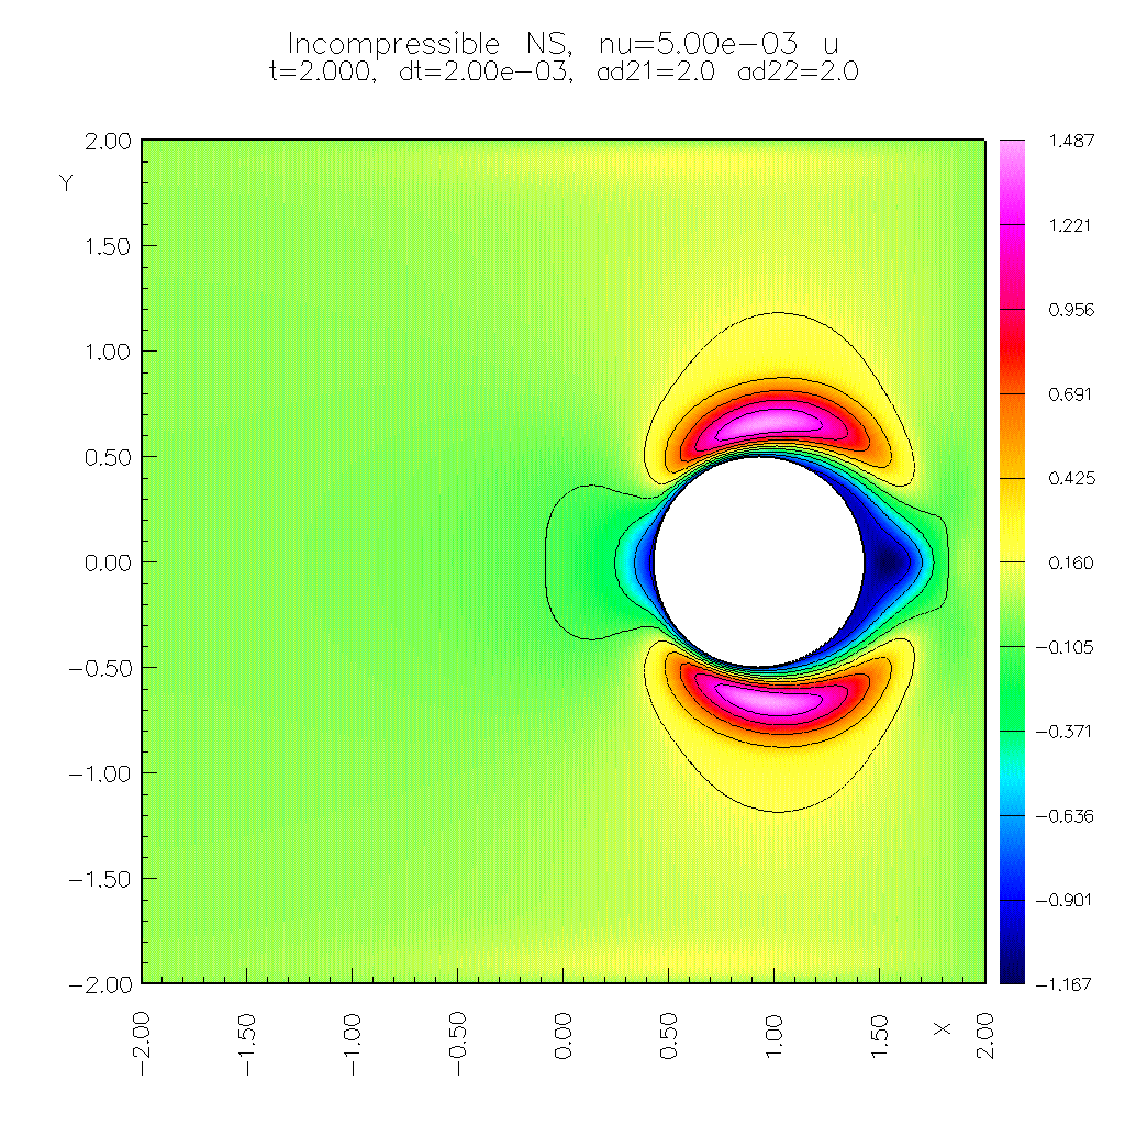
\includegraphics[width=\figWidth]{figures/collide6-u-2p0}  
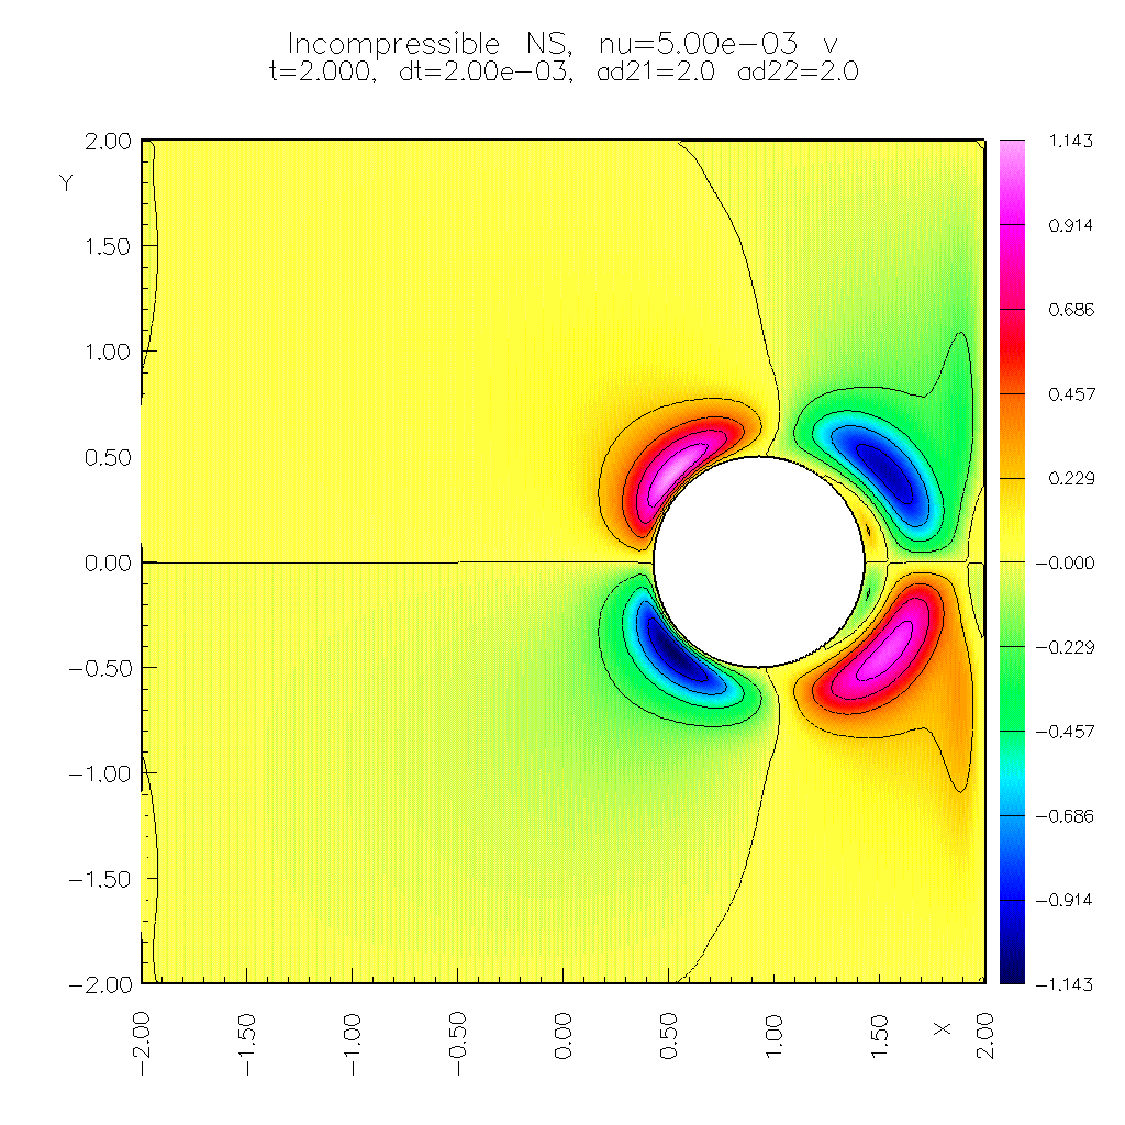
\includegraphics[width=\figWidth]{figures/collide6-v-2p0}  
\end{center}
\caption{Cylinder hitting a wall, $\nu=.005$, solution at times $.5$, $1.4$ and $2.0$} 
\end{figure}
}


\begin{figure}
\begin{center}
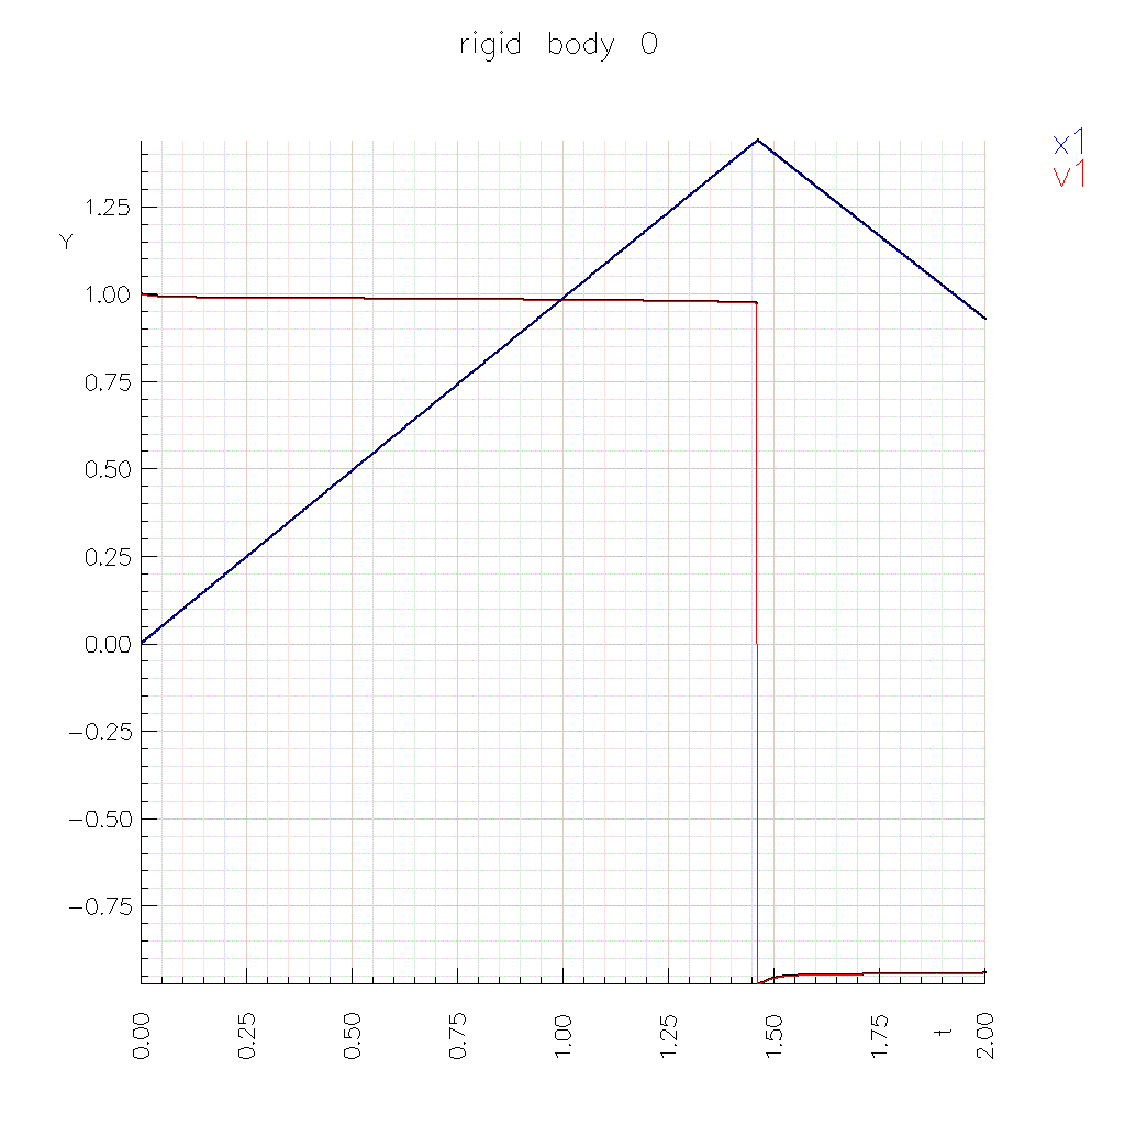
\includegraphics[width=.45\linewidth]{figures/collide6-rb-x1}  
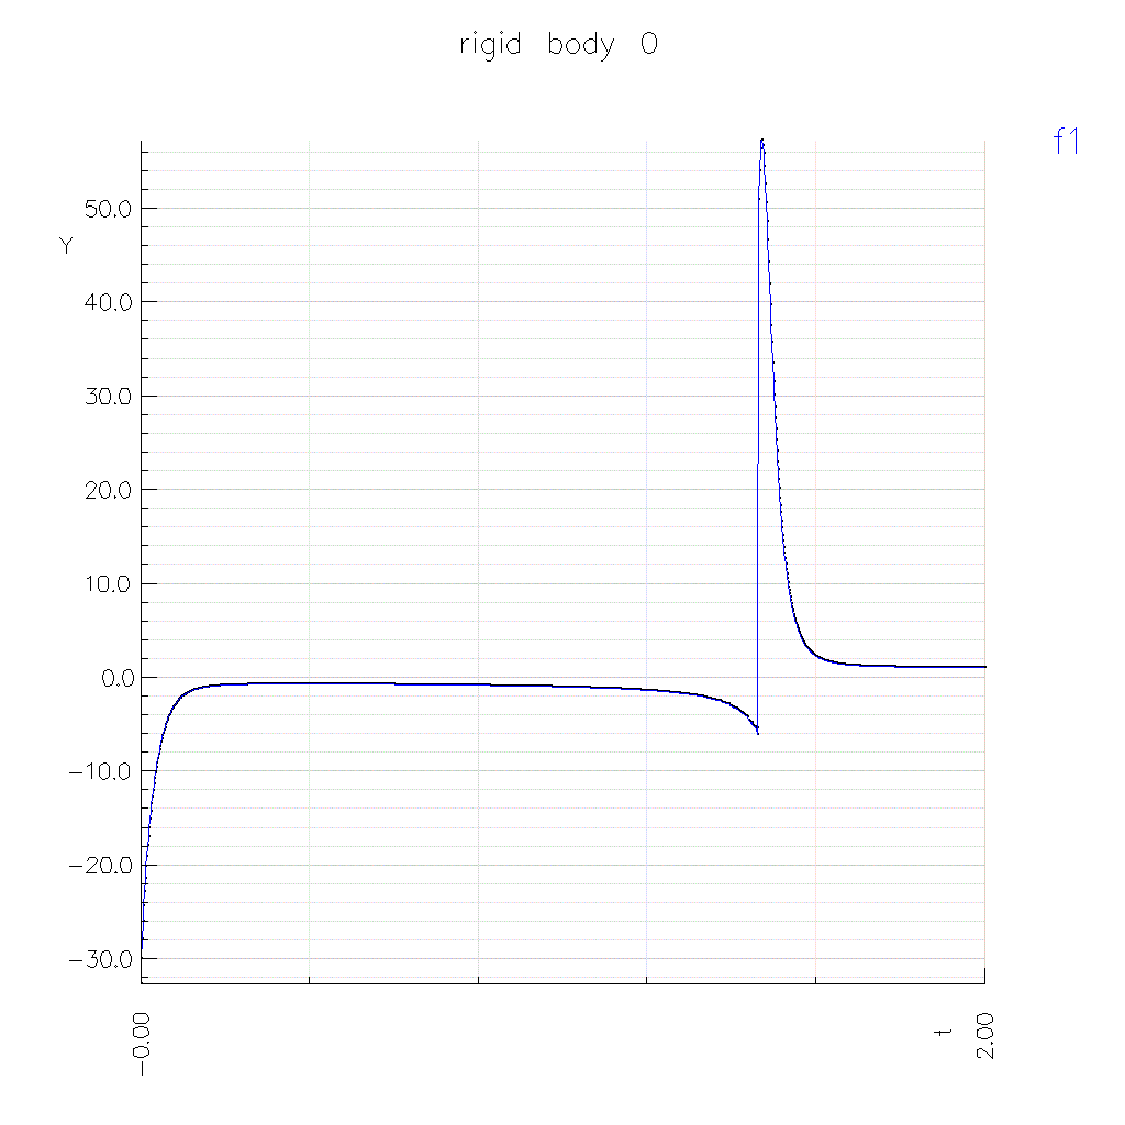
\includegraphics[width=.45\linewidth]{figures/collide6-rb-f1}  
\end{center}
\caption{Cylinder hitting a wall, $\nu=.005$, position of the centre of mass and the force on the cylinder.}
\end{figure}


% ----------------------------------------------------------------------------------------------------------



